\section{Численное моделирование работы искусственного сердечного
клапана}\label{ux447ux438ux441ux43bux435ux43dux43dux43eux435-ux43cux43eux434ux435ux43bux438ux440ux43eux432ux430ux43dux438ux435-ux440ux430ux431ux43eux442ux44b-ux438ux441ux43aux443ux441ux441ux442ux432ux435ux43dux43dux43eux433ux43e-ux441ux435ux440ux434ux435ux447ux43dux43eux433ux43e-ux43aux43bux430ux43fux430ux43dux430}

В данной работе рассмотрена математическая модель, описывающая динамику
искусственного сердечного клапана, движущегося под воздействием течение
неоднородной несжимаемой жидкости с переменной вязкостью, а также метод
ее численного решения. Приведены результаты моделирования работы
трехстворчатого клапана, включая динамику движения лепестков, для разных
геометрий (клапан идеальной формы, а также клапан, полученный
сканированием биопротеза ``Юнилайн''), напряжение, возникающее на
фиброзном кольце и лепестках, а также динамику распространения примесей.

\subsection{Введение}\label{ux432ux432ux435ux434ux435ux43dux438ux435}

На сегодняшний день исследования в области сердечно-сосудистой системы
человека востребованы как никогда. Это связано с двумя основными
причинами:

\begin{itemize}
\item
  сердечно-сосудистые заболевания становятся все более
  распространненными в силу ряда социальных причин (экономические
  изменения, урбанизация и проч. приводят к изменению образа жизни
  многих людей) и увеличения влияния факторов риска (например,
  уменьшение физической активности) {[}1{]}. Каждый год в мире
  проводится примерно 250 000 операций по восстановлению или замене
  поврежденных сердечных клапанов, и наблюдается тенденция к росту этого
  числа {[}2{]}.
\item
  развитие технологий, используемых в медицине, позволяет получать более
  точные экспериментальные данные и выявлять новые явления и процессы,
  требующие объяснения.
\end{itemize}

Искусственные сердечные клапана являются одними из самых сложных
инструментов, используемых в кардио хирургии. Они достаточно эффективно
позволяют бороться с заболеваниями и повреждениями естесственных
клапанов, но при этом вносят новые проблемы. Например, механические
клапаны обладают высокой надежностью и долговечностью, но могут
приводить к сильным деформациям потока, формированию сгустков кровяных
клеток. Биологические клапаны лишены этого недостатка, однако они менее
долговечны. математическое моделирование работы искусственного клапана
может позволить получить более глубокое понимание происходящих процессов
в нём и тем самым найти пути усовершенствования их конструкции.

В силу важности данной темы существует множество исследований по
моделированию и численному решению работы сердечного клапана.
Большинство из них акцентируют внимание только на самом клапане, анализе
его поведения, деформации и напряжениях, возникающих под воздействием
давления {[}3{]}, {[}4{]}. При этом поток жидкости, приводящий в
движение клапан, рассматривается достаточно упрощенно. Для того, чтобы
построить более полную модель, необходимо рассматривать полноценное
взаимодействие жидкости и клапана. Существует два основных подхода,
которые позволяют это сделать.

Первый подход связан с использованием конечно-элементных методов
({[}5{]}, {[}6{]}, {[}7{]}). Используя их, можно хорошо учитывать
сложную геометрию сердца, однако необходимость учитывать взаимодействие
жидкости и гибких стенок приводит к постоянному перестраиванию расчетной
сетки, чтобы удовлетворять меняющейся геометрии исследуемого объекта.
Это приводит к существенным затратам времени и вычислительных ресурсов.

Широко распространен другой подход, который связан с методом погруженной
границы ({[}8{]}, {[}9{]}, {[}10{]}). Он может применяться в задачах со
сложной геометрией, но при этом не требует модификации сетки, и
позволяет моделировать сколь угодно тонкие лепестки клапана.

В данной работе мы используем именно этот подход, и предлагаем описывать
движение крови в упругих крупных кровеносных сосудах и искусственном
сердечном клапане как трехмерное нестационарное течение вязкой
несжимаемой жидкости с переменной плотностью и вязкостью (см. {[}11{]},
{[}12{]}, {[}13{]}, {[}14{]}). Таким образом, целью работы является
построение математической модели и метода решения задачи о движении
створок искусственного клапана внутри кровеносного сосуда с учетом
неоднородной структуры крови, а также о движении примеси (форменных
элементов) внутри сосуда.

\subsection{Постановка
задачи}\label{ux43fux43eux441ux442ux430ux43dux43eux432ux43aux430-ux437ux430ux434ux430ux447ux438}

Как известно {[}15{]}, стенки сосуда и створки клапана состоят из
большого количества коллагеновых волокон, и изменяют свою форму в
зависимости от течения крови. Створки клапана исключительно тонки, их
основание крепятся к жесткому кольцу из фиброзной ткани. Кровь состоит
из плазмы и взвешенных в ней форменных элементов, которые составляют
примерно 45\% от всего объема и, вообще говоря, является неньютоновской
жидкостью.

\begin{figure}[htbp]
\centering
\includegraphics{heart_scheme.png}
\caption{\label{fig:heart_scheme}Изображение аортального клапана и его
расположение в сердце}
\end{figure}

Размеры форменных элементов очень малы по сравнению с размерами сосуда
(например, диаметр аорты \(\sim 3 \cdot 10^{-2}\text{м}\), а диаметр
эритроцита \(\sim 6 \cdot 10^{-9}\text{м}\)). Это позволяет моделировать
кровь как вязкую, несжимаемую неоднородную двухкомпонентную жидкость с
переменной вязкостью. Стенки сосуда и створки клапана -- как
непроницаемую для жидкости поверхность, обладающую некоторой жесткостью.
Под воздействием давления жидкости створки клапана деформируются. Как
было сказано выше, кровь является неньютоновской жидкостью, однако, как
показано в {[}16{]}, отдельно плазма ведет себя как ньютоновская
жидкость. При этом, реологические свойства крови очень зависят от
скорости сдвига (shear rate), и для большей части сердечного цикла в
артериях и желудочках сердца его величина превышает пороговое значение
\(50\; \text{сек}^{-1}\), поэтому кровь может рассматриваться как
ньютоновская жидкость.

\begin{figure}[htbp]
\centering
\includegraphics{aorta_valve_scheme.png}
\caption{\label{fig:aorta_valve_scheme}Изображение границ расчетной
области}
\end{figure}

Так как источником движения крови в сосудах является давление,
создаваемое сокращением сердца, то задачу о ее движении опишем следующей
нестационарной системой дифференциальных уравнений Навье-Стокса
{[}11{]}:

\begin{equation}\frac{\partial \vec{u}}{\partial t} + (\vec{u} \cdot \nabla) \vec{u} = - \frac{1}{\rho} \nabla p + \nabla \sigma + \vec{f}\label{eq:navier_stokes:motion}\end{equation}

\begin{equation}\frac{\partial \rho}{\partial t} + \nabla \cdot (\rho \vec{u}) = 0\label{eq:navier_stokes:continuity}\end{equation}

с начальными и краевыми условиями:

\begin{equation}\vec{u}(\bar{x}, 0) = \vec{u}_0 \qquad \vec{u}|_{\Gamma_1, \Gamma_4} = \vec{u}_b \qquad u_{\Gamma_2, \Gamma3} = 0\label{eq:navier_stokes:velocity_conditions}\end{equation}

\begin{equation}p_{\Gamma_2} = p_{in} \qquad p_{\Gamma_3} = p_{out}\label{eq:navier_stokes:pressure_conditions}\end{equation}

где \(\bar{x}=(x,y,z) \in \Omega\), \(\vec{u}=(u,v,w)\) - вектор
скорость, \(u, v, w\) - \(x\)-, \(y\)-, \(z\)-компонента вектора
скорости, \(\vec{u}_b\) - скорость движения лепестков клапана под
воздействием деформации, \(\rho=\rho(\bar{x}, t)\) - плотность,
\(p=p(\bar{x}, t)\) - давление,
\(\sigma = \mu (\nabla \vec{u} + (\nabla \vec{u})^T)\) - вязкий тензор
напряжений, \(\mu = \mu(\bar{x}, t)\) - вязкость жидкости,
\(\vec{f} = \vec{f}(\bar{x}, t)\) - вектор массовых сил. Область
\(\Omega\) представляет собой сосуд с границами
\(\Gamma = \Gamma_1 \cup \Gamma_2 \cup \Gamma_3 \cup \Gamma_4\), где
\(\Gamma_1\) - стенки кровеносного сосуда, \(\Gamma_2\) and \(\Gamma_3\)
- области втекания/вытекания, \(\Gamma_4\) - лепестки клапана (см рис.
\ref{fig:aorta_valve_scheme}).

Отсутствие задания одной компоненты вектора скорости на участках
втекания-вытекания является одной из проблем при численном решении задач
подобного типа. Она решается с помощью использования исходных уравнений
(\ref{eq:navier_stokes:motion}) - (\ref{eq:navier_stokes:continuity}) на
границах \(\Gamma_2\) и \(\Gamma_3\) для вычисления недостающих
компонент вектора скорости (подробнее см. {[}11{]}, {[}12{]}).

Как показано в {[}11{]}, для того, чтобы моделировать движение
неоднородной жидкости (плазма и примеси), можно добавить к системе
уравнений (\ref{eq:navier_stokes:motion}),
(\ref{eq:navier_stokes:continuity}) уравнение переноса концентрации:

\begin{equation}\frac{\partial c}{\partial t} + \vec{u} \cdot \nabla c = 0\label{eq:convection}\end{equation}

с начальными условиями:

\begin{equation}c(\bar{x}, 0) = c_0(\bar{x}), \bar{x} \in \Omega\label{eq:convection:conditions}\end{equation}

с краевыми условиями для области втекания:

\begin{equation}c(\bar{x}, t)|_{\Gamma_2} = c_s(\bar{x}, t)\label{eq:convection:conditions}\end{equation}

и связать переменную плотность и вязкость с концентрацией примеси
следующими линейными соотношениями:

\begin{equation}\mu = c (\mu_2 - \mu_1) + \mu_1\label{eq:viscosity}\end{equation}

\begin{equation}\rho = c (\rho_2 - \rho_1) + \rho_1\label{eq:density}\end{equation}

Т.о. мы получим математическую модель течения крови, которая отражает ее
сложную структуру, а также позволяет легко расширить это описание для
описания большего количества компонент и более сложных условий
зависимости плотности и вязкости от концентрации.

Для того, чтобы иметь возможность моделировать движение тонких гибких
клапанов, необходимо расширить полученную модель, добавив в нее силы,
возникающие при деформации лепестков клапана и стремящиеся вернуть их в
равновесное состояние. При этом мы можем моделировать стенки сосуда
таким же образом, что и клапан, учитывая при этом, что створки клапана
деформируются гораздо сильнее, чем стенки сосуда.

Для описания сил, возникающих при деформации клапана, воспользуемся
следующей формулой {[}8{]}, {[}9{]}:

\begin{equation}F = \frac{\partial}{\partial s} T \tau + \frac{\partial^2}{\partial s} \left( k \cdot \left(\frac{\partial^2 X^0}{\partial s^2} - \frac{\partial^2 X}{\partial s^2} \right) \right)\label{eq:resulting_force}\end{equation}

где \(k = E \cdot I\), \(E\) - модуль упругости, \(I\) - момент инерции
поперечного сечения, \(\frac{\partial^2 X^0}{\partial s^2}\),
\(\frac{\partial X}{\partial s^2}\) - отклонение погруженной границы от
равновесного положения в начальный и текущий момент времени.

Как показано в {[}8{]}, для того, чтобы описать взаимодействие потока
жидкости и клапана, необходимо ввести в рассмотрение прямоугольную
область \((x, y, z) = \bar{x} \in \tilde{\Omega}\), так что
\(\Omega \in \tilde{\Omega}\), а также область
\((q, r, s) = \bar{q} \in \Gamma\), которая соответствует точкам клапана
в лагранжевых координатах. После этого, опишем взаимодействи с помощью
следующих уравнений:

\begin{equation}\frac{\partial X}{\partial t}(\bar{q}, t) = \int_{\Omega} \vec{u}(\bar{x}, t) \cdot \delta (x - X(\bar{q}, t))\; d\bar{x}\label{eq:interaction:velocity}\end{equation}

\begin{equation}\vec{f}(\bar{x}, t) = \int_{\Gamma} \vec{F}(\bar{q}, t) \cdot \delta (x - X(\bar{q}, t))\; d\bar{q}\label{eq:interaction:force}\end{equation}

где \(\delta\) - дельта функция Дирака, \(F\) - плотность силы
деформации. Уравнения \ref{eq:interaction:velocity},
\ref{eq:interaction:force} и позволяют переходить от эйлеровых к
лагранжевым координатам.

Таким образом, мы построили модель, описывающую движение вязкой
неоднородной несжимаемой жидкости внутри сосуда с клапаном. В этой
модели состояние жидкости и форма поверхностей
\(\Gamma_1 \cup \Gamma_4\) определяются независимо друг от друга, а
влияние створок клапана на течение отражено с помощью соотношения
(\ref{eq:interaction:force}) между вектором массовых сил
\(\vec{f}(\bar{x}, t)\) уравнения (\ref{eq:navier_stokes:motion}) и
силой сопротивления деформации \(F=F(\bar{q}, t)\) из уравнения
(\ref{eq:resulting_force}).

\section{Метод
решения}\label{ux43cux435ux442ux43eux434-ux440ux435ux448ux435ux43dux438ux44f}

Как было сказано выше, в данной работе используется метод погруженной
границы {[}8{]}. В соответствии с этим методом, будем рассчитывать
течение жидкости в параллелепипеде \(\tilde{\Omega}\), который включает
в себя \(\Omega\). На границах \(\tilde{\Omega}\) задано условие
прилипания. Для расчета течения жидкости будем использовать
прямоугольную равномерную разнесенную сетку \(\tilde{\Omega_h}\) с
шагами \(h_{xi}, h_{yj}, h_{zk}\) и шахматным расположением узлов, где
давление, дивергенция скорости и концентрация определяются в центре
ячейки, а компоненты вектора скорости и внешних сил -- на границах. Для
определения деформации поверхности \(\Gamma_1 \cup \Gamma_4\) введем
дополнительную область \(\tilde{\Gamma}\) системой координат,
соотнесенной со стенками сосуда и створками клапана. В области
\(\tilde{\Gamma}\) точкам на \(\Gamma_1 \cup \Gamma_4\). Алгоритм
решения состоит из нескольких шагов: на сетке \(\tilde{\Omega_h}\)
решаем задачу
(\ref{eq:navier_stokes:motion})-(\ref{eq:navier_stokes:pressure_conditions});
затем решаем уравнение конвекции (\ref{eq:convection}) т.е. определяем
концентрацию примеси в области решения и пересчитываем значение
плотности и вязкости. После этого используем формулы
(\ref{eq:resulting_force}) и (\ref{eq:interaction:velocity}),
(\ref{eq:interaction:force}) для определения положения створок клапана и
формы

\begin{figure}[htbp]
\centering
\includegraphics{aorta_valve_computation_scheme.png}
\caption{\label{fig:aorta_valve_computation_scheme}Расчетные области,
используемые в методе погруженной границы}
\end{figure}

Поставленная дифференциальная задача (\ref{eq:navier_stokes:motion}) --
(\ref{eq:density}) решается методом конечных разностей. Для решения
(\ref{eq:navier_stokes:motion}) --
(\ref{eq:navier_stokes:pressure_conditions}) будем использовать схемы
расщепления по физическим факторам {[}17{]}:

\begin{equation}\frac{u^* - u^n}{\triangle t} = - (u^n \cdot \nabla) u^* - \frac{1}{\rho}
\nabla \sigma + f^n\label{eq:splitting:intermediate_velocity}\end{equation}

\begin{equation}\rho \triangle p^{n+1} - \nabla \rho \cdot p^{n+1} = \frac{\rho^2 \nabla
u^*}{\triangle t} \label{eq:splitting:poisson}\end{equation}

\begin{equation}\frac{u^{n+1} - u^*}{\triangle t} = - \frac{1}{\rho} \triangle p^{n+1} \label{eq:splitting:velocity}\end{equation}

Численная реализация схемы состоит из 3-х этапов. Сначала по известным
значениям скорости с предыдущего временного слоя находится промежуточное
поле \(u^*\). Для этого уравнение
(\ref{eq:splitting:intermediate_velocity}) решается методом
стабилизирующей поправки {[}18{]}. Затем, путем численного решения
(\ref{eq:splitting:poisson}) с использованием метода бисопряженных
градиентов, определяется новое поле давления. И на последнем этапе
восстанавливается окончательное поле вектора скорости по явным формулам
(\ref{eq:splitting:velocity}).

После нахождения параметров течения жидкости необходимо вычислить новые
значения плотности и вязкости. Для этого, используя полученные значения
компонент скорости, делается шаг по времени для уравнения конвекции
(\ref{eq:convection}), и производится пересчет значений плотности и
вязкости по формулам (\ref{eq:viscosity}), (\ref{eq:density}).

Далее нам необходимо определять деформацию стенок сосуда и створок
клапана под воздействием жидкости, а также распределение массовых сил fв
уравнении движения жидкости исходя из возникшей деформации. Используя
уравнения (\ref{eq:interaction:velocity}) --
(\ref{eq:interaction:force}), которые численно интегрируются с помощью
какой-либо квадратурной формулы, и уравнение (\ref{eq:resulting_force}),
мы можем рассчитать деформацию, которой подвергаются стенки сосуда и
клапан при данном давлении жидкости и возникающую силу сопротивления
\(F\). После этого пересчитываем массовые силы \(f\) и переходим на
следующий шаг по времени.

\section{Результаты}\label{ux440ux435ux437ux443ux43bux44cux442ux430ux442ux44b}

Приведем резульаты некоторых результатов, полученных в рамках данной
работы. Расчеты проводились для случаев постоянной и переменной
плотности и вязкости в безразмерных величинах. Для клапана
использовались две геометрии - идеальный клапан упрощенной формы и
клапан, полученный сканированием реального биопротеза ``Юнилайн''
{[}19{]}. В качестве сосуда для всех расчетов используется круговой
цилиндр с длинной \(l=1\), радиусом \(r=0.11\) и жесткостью стенок
\(k=1 \cdot 10^{3}\). Для створок клапана заданы коэффициенты
сопротивления растяжению \(k_s = 5 \cdot 10^{3}\) и скручиванию
\(k_b = 2 \cdot 10^{3}\). Перепад давления \(p_{in} - p_{out}\)
периодически меняется от 0 до 6. Область \(\tilde{\Omega}\) имеет
параметры \(10 \times 0.5 \times 0.5\), шаги по пространственной сетке
\(\tilde{\Omega_h}\) \(h_x = h_y = h_z = 0.01\), шаг по времени
\(\triangle t = 0.01\).

На рис. \ref{fig:ideal_valve_stress} показана динамика движения одного
лепестка идеального трехстворчатого клапана под воздействием жидкости с
постоянной вязкостью и плотностью
\(\rho_1=\rho_2=1, \mu_1=\mu_2=1 \cdot 10^{-2}\), а также распределение
напряжения по поверхности.

\begin{figure}[htbp]
\centering
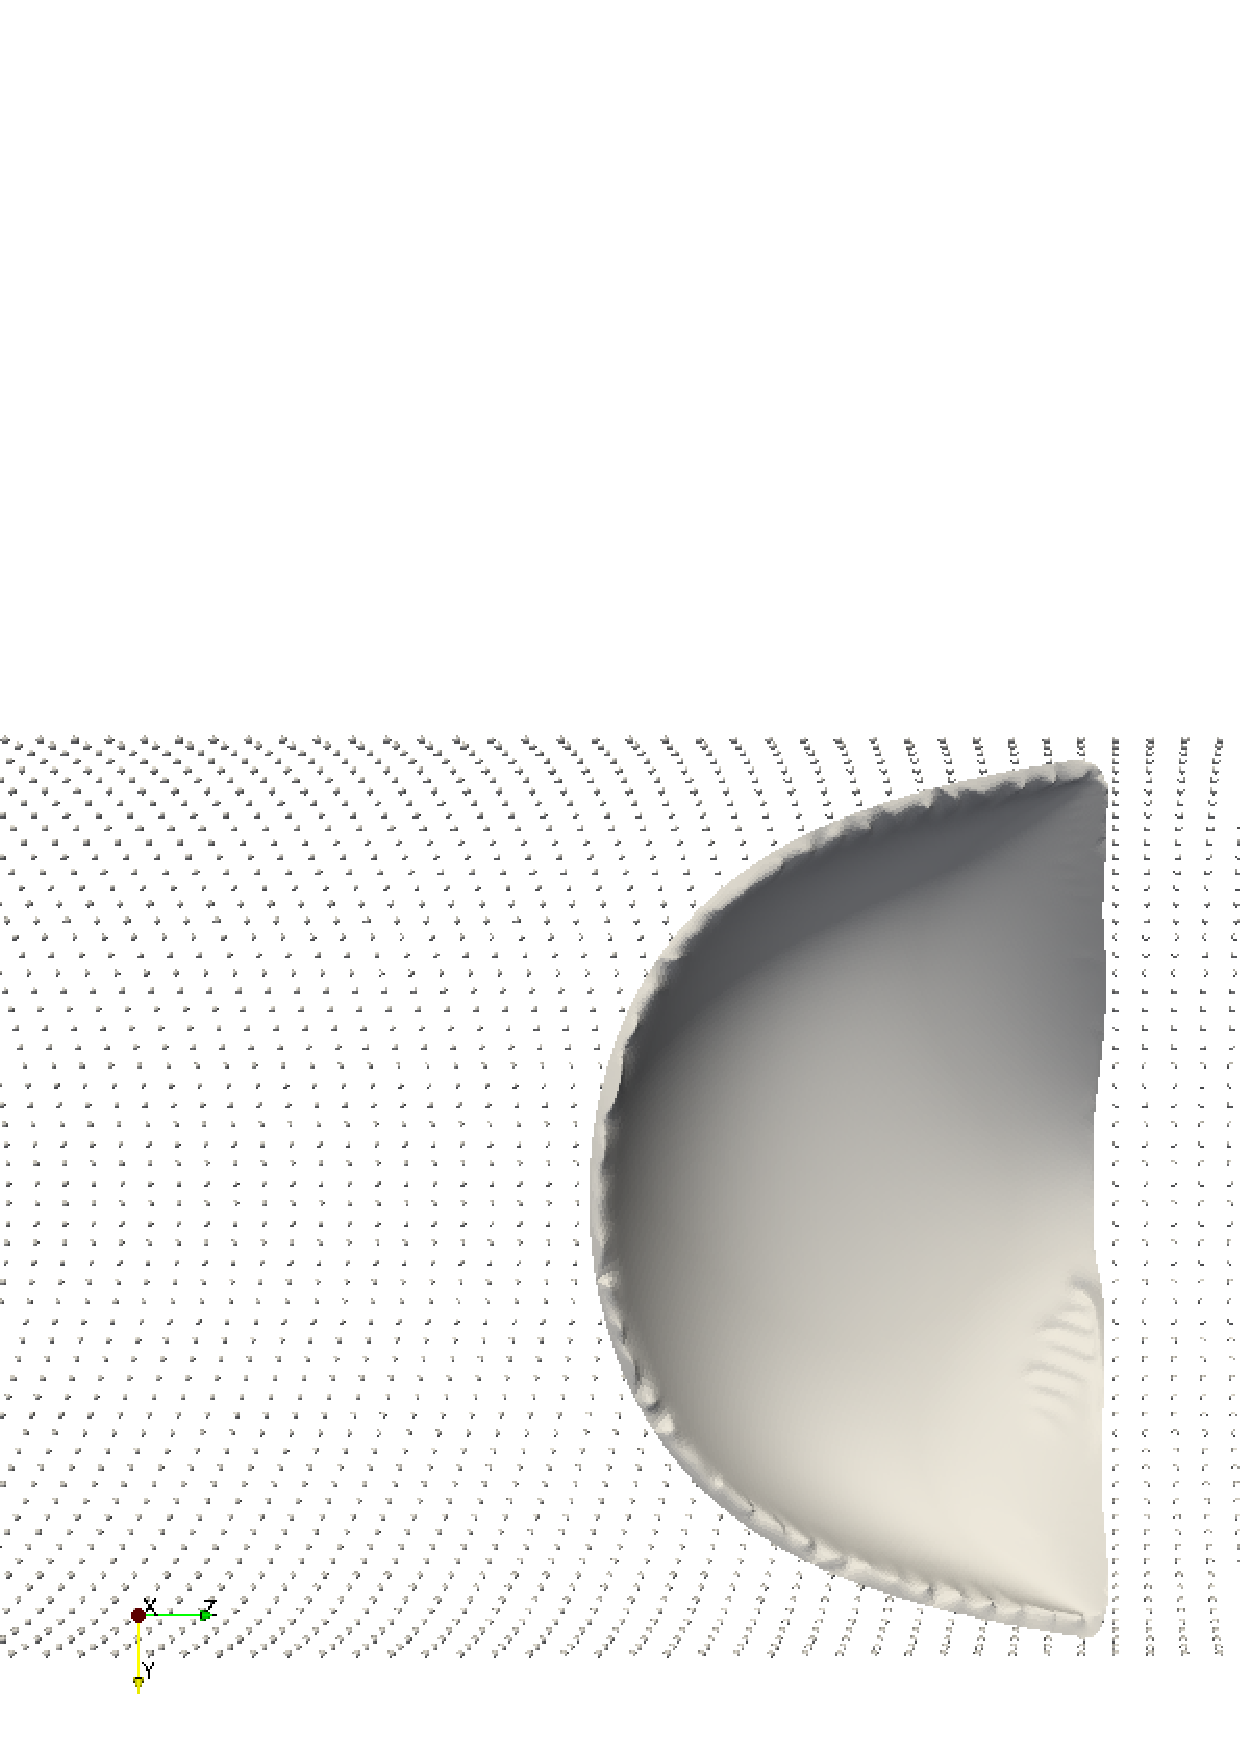
\includegraphics{ideal_valve_stress_1.png}
\caption{}
\end{figure}

\begin{figure}[htbp]
\centering
\includegraphics{ideal_valve_stress_2.png}
\caption{}
\end{figure}

\begin{figure}[htbp]
\centering
\includegraphics{ideal_valve_stress_3.png}
\caption{\label{fig:ideal_valve_stress}Распределение напряжение по
поверхности лепестка во времена t=0, t=0.4, t=0.8. Точками обозначены
стенки сосуда}
\end{figure}

Как видно из рис. \ref{fig:ideal_valve_stress}, больше поверхностного
напряжения возникает в двух областях - на конце лепестка, т.к. это самая
гибкая его часть, которая подвержена наибольшим деформациям скручивания,
и в области крепления лепестка к фиброзному кольцу, т.к. там возникает
наибольшая деформация растяжения в силу фиксированного расположения.

На рис. \ref{fig:uniline_dynamics} представлена динамика движения для
клапана ``Юнилайн'', который двигается под воздействием движения
жидкости с постоянной вязкостью и плотностью
\(\rho_1=\rho_2=1, \mu_1=\mu_2=1 \cdot 10^{-2}\).

\begin{figure}[htbp]
\centering
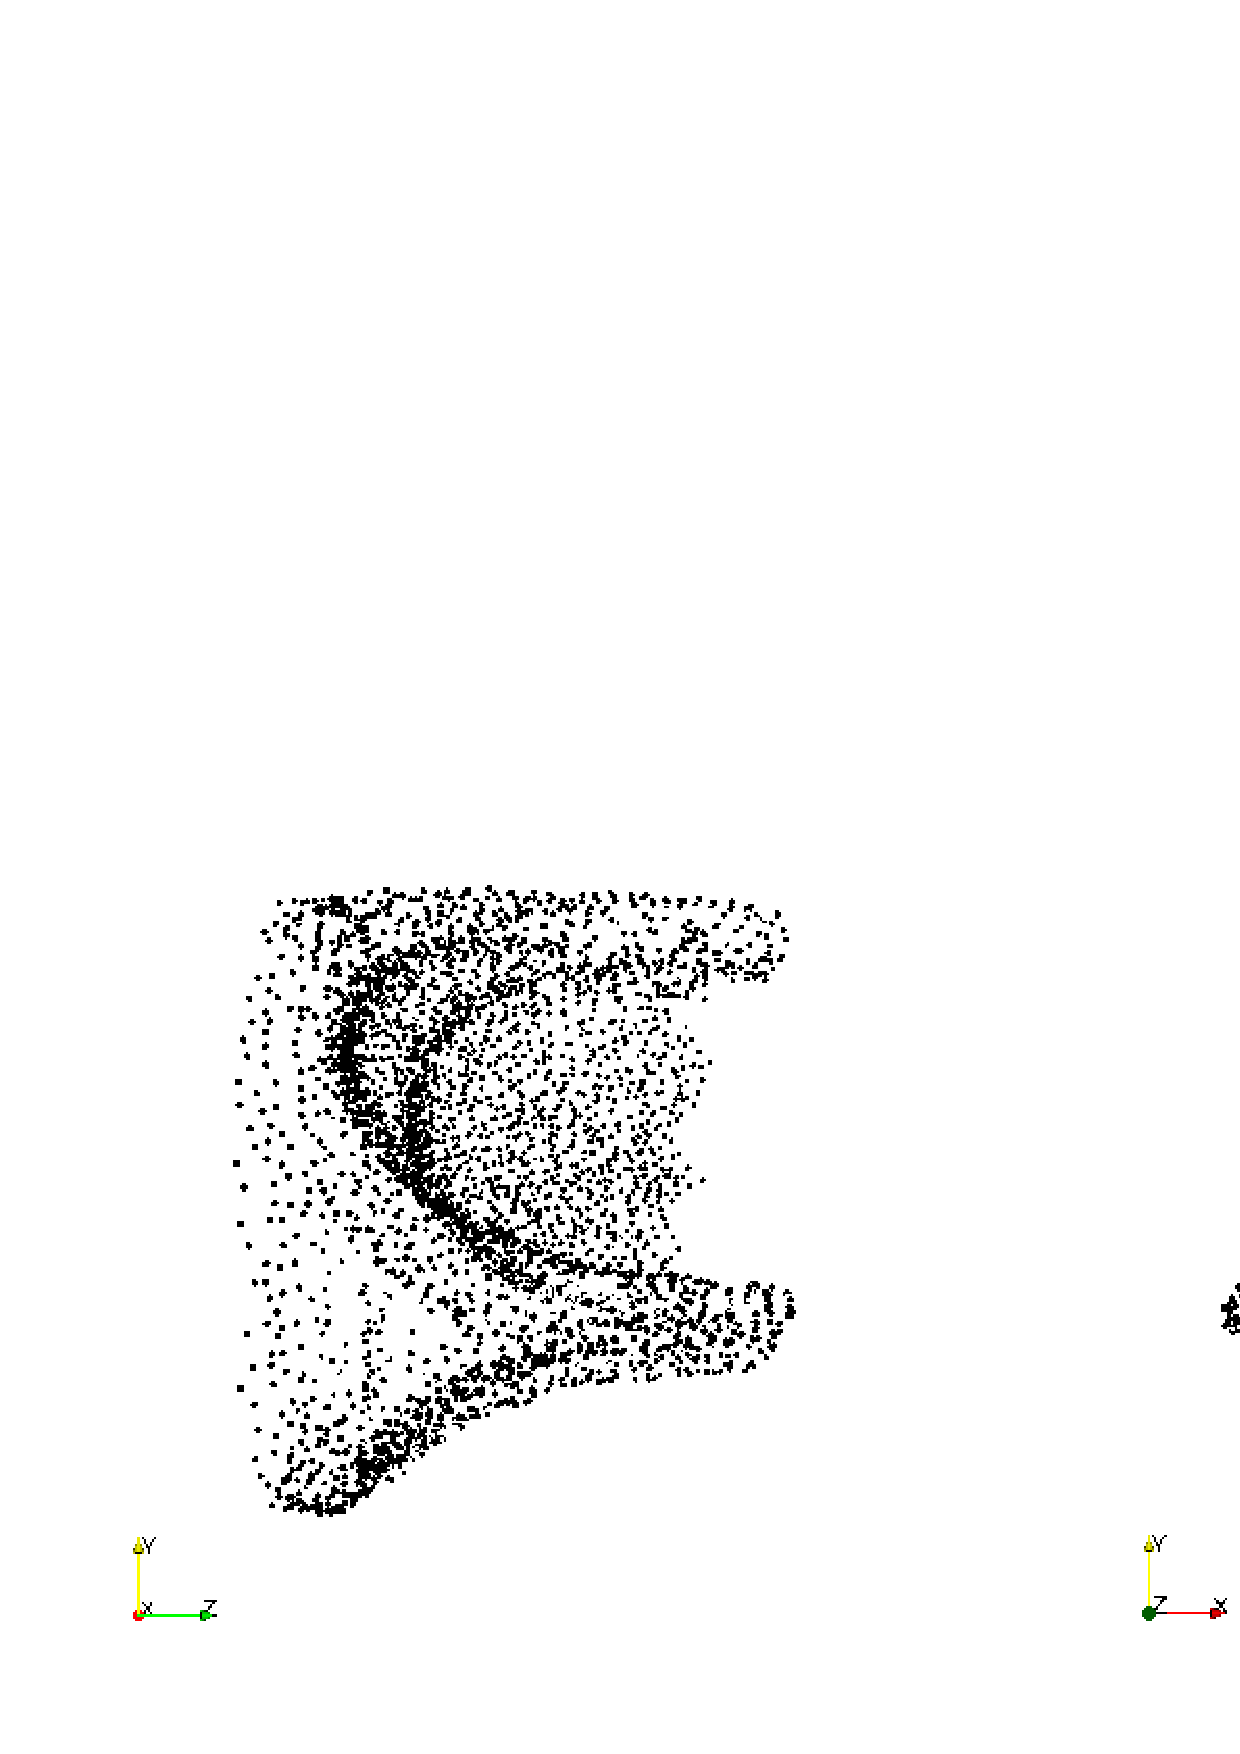
\includegraphics{uniline_dynamics_11.png}
\caption{}
\end{figure}

\begin{figure}[htbp]
\centering
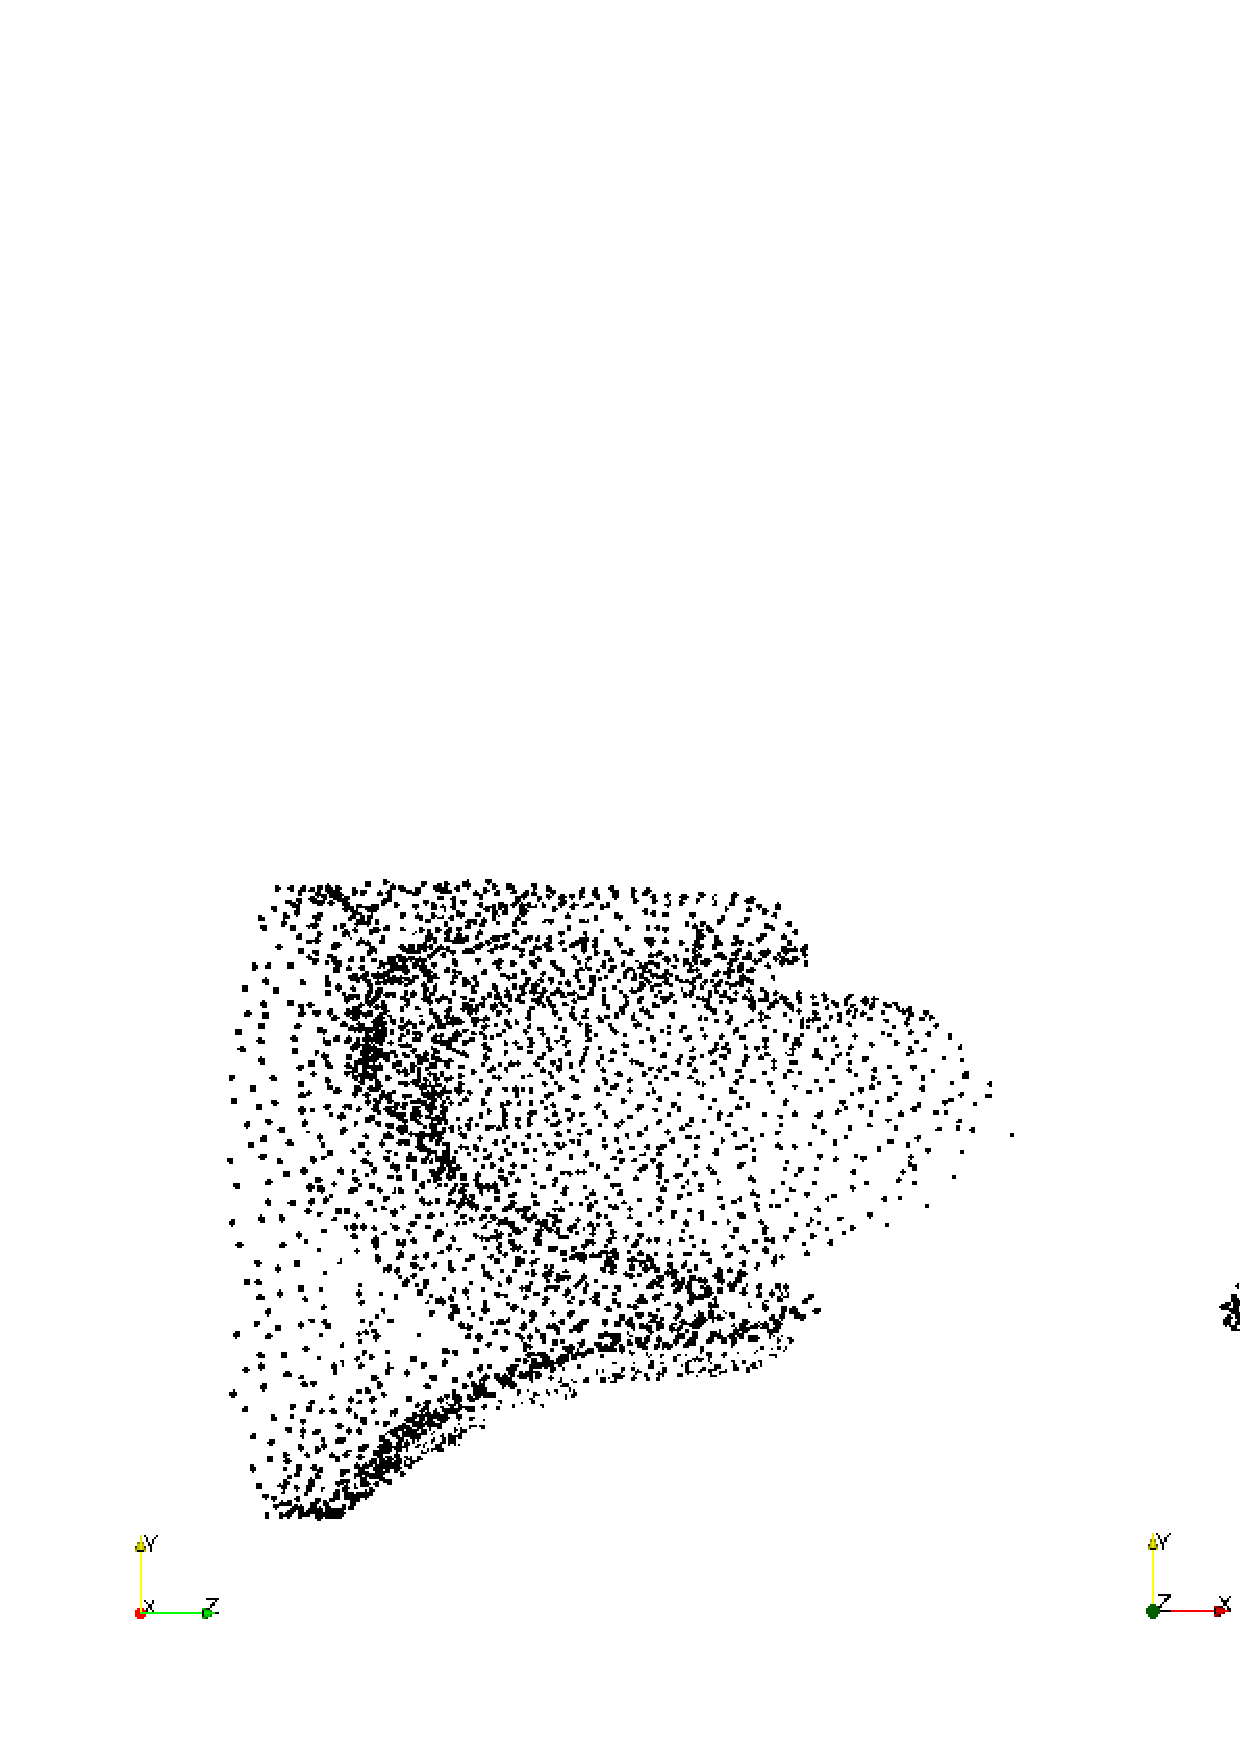
\includegraphics{uniline_dynamics_22.png}
\caption{}
\end{figure}

\begin{figure}[htbp]
\centering
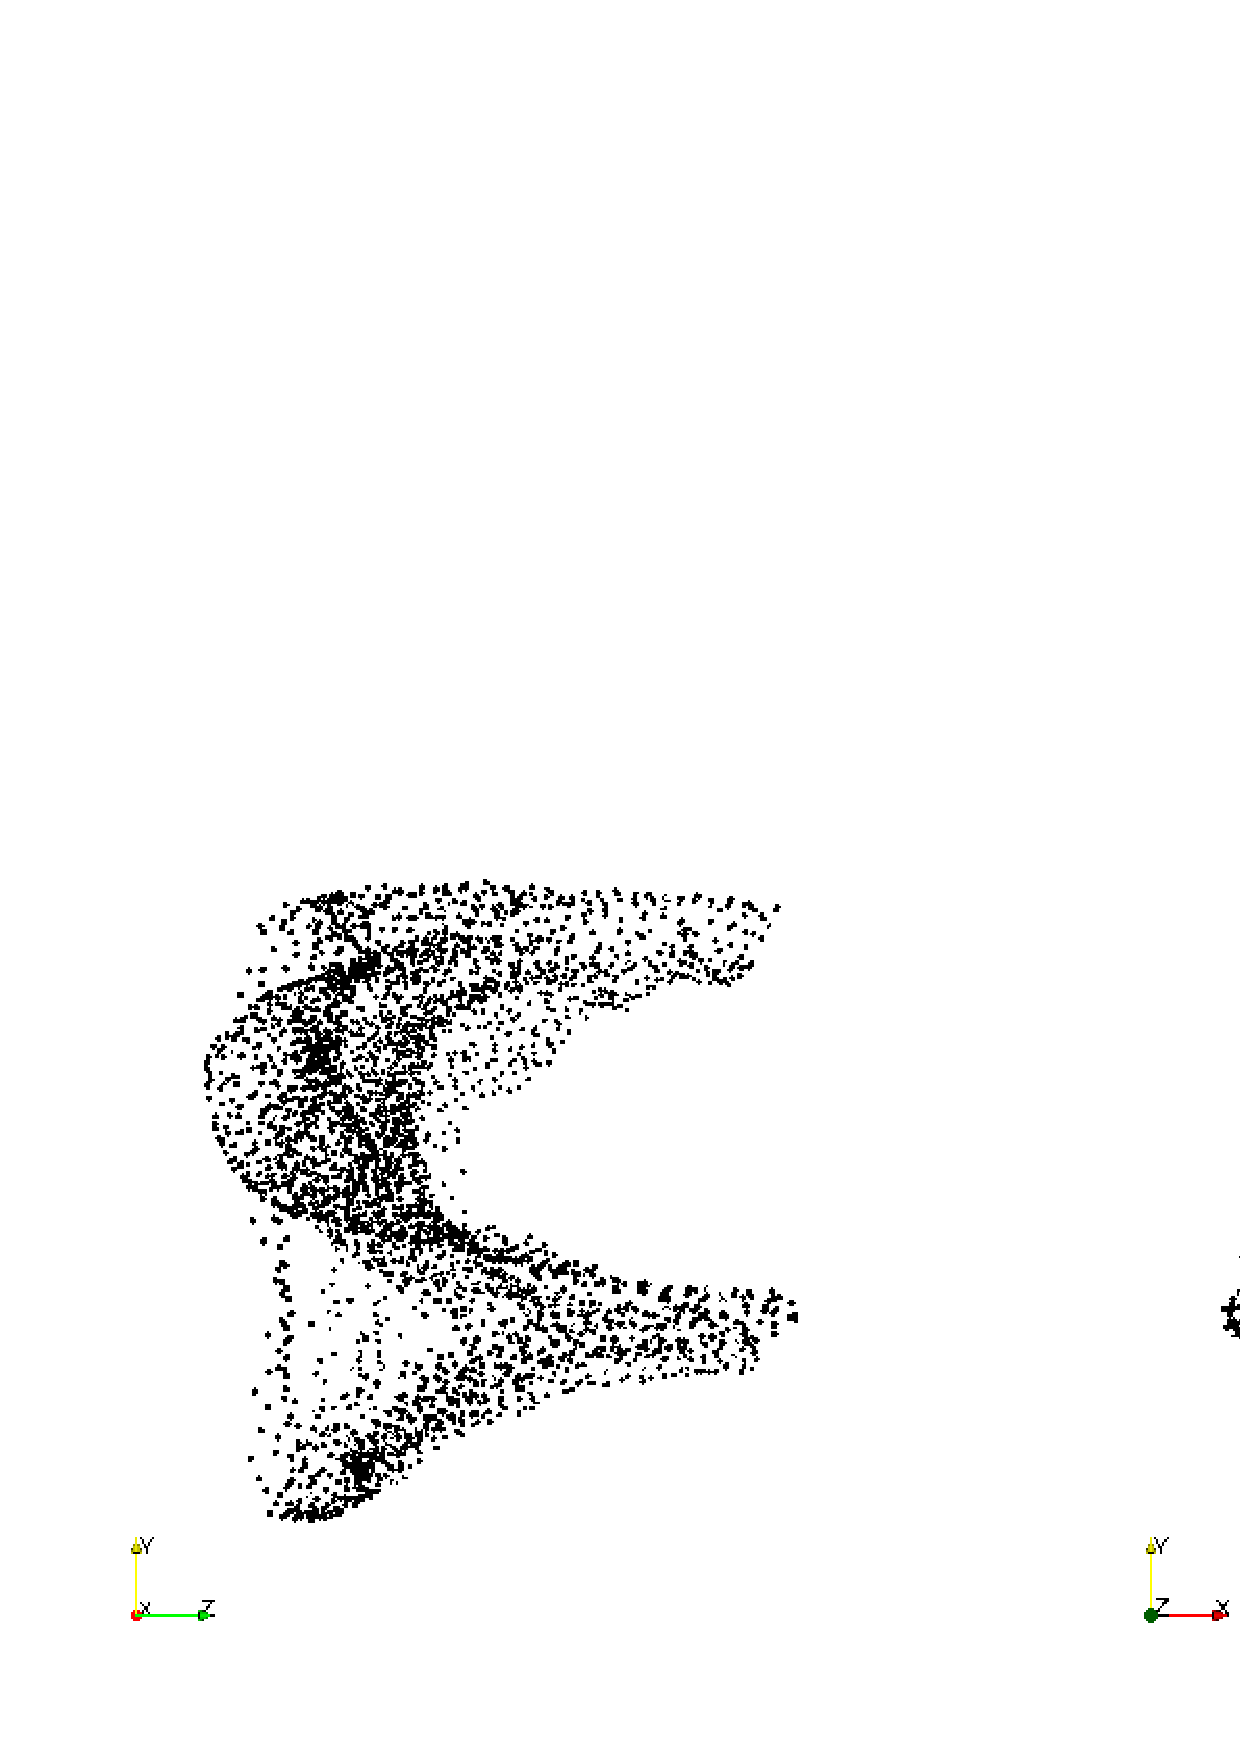
\includegraphics{uniline_dynamics_33.png}
\caption{\label{fig:uniline_dynamics}Работа клапана во времена t=0,
t=0.5, t=1.8. Точками обозначена поверхность фиброзного кольца и
лепестков клапана}
\end{figure}

На рис. \ref{fig:uniline_stress} представлена динамика движения и
распределение поверхностного напряжения для лепестка клапана
``Юнилайн'', который двигается под воздействием движения жидкости с
постоянной вязкостью и плотностью
\(\rho_1=\rho_2=1, \mu_1=\mu_2=1 \cdot 10^{-2}\).

\begin{figure}[htbp]
\centering
\includegraphics{uniline_stress_1.png}
\caption{}
\end{figure}

\begin{figure}[htbp]
\centering
\includegraphics{uniline_stress_2.png}
\caption{}
\end{figure}

\begin{figure}[htbp]
\centering
\includegraphics{uniline_stress_3.png}
\caption{\label{fig:uniline_stress}Распределение напряжение по
поверхности лепестка во времена t=0, t=0.4, t=0.8. Точками обозначена
поверхность фиброзного кольца}
\end{figure}

Рис. \ref{fig:uniline_stress} показывает небольшую ассиметрию
распределения напряжения, связанную с исходной ассиметрией клапана.
Помимо этого, в отличии от клапана идеальной формы, в области крепления
лепестка к фиброзному кольцу не происходит значительного увеличения
напряжения.

\begin{figure}[htbp]
\centering
\includegraphics{valve_points.png}
\caption{\label{fig:points_scheme}Схема расположения точек на фиброзном
кольце}
\end{figure}

На рис. \ref{fig:fibrouse_forces} показано графики зависимости
поверхностного напряжения от времени для трех точек в разных частях
фиброзного кольца. ``Активная точка'' находится на одной из осей кольца,
рядом с областью крепления лепестка. ``Точка на границе'' тоже
располагается в области крепления, но на удалении от осей. ``Пассивная
точка'' располагается на внешней, наименее подвижной части кольца (см.
рис. \ref{fig:points_scheme}).

\begin{figure}[htbp]
\centering
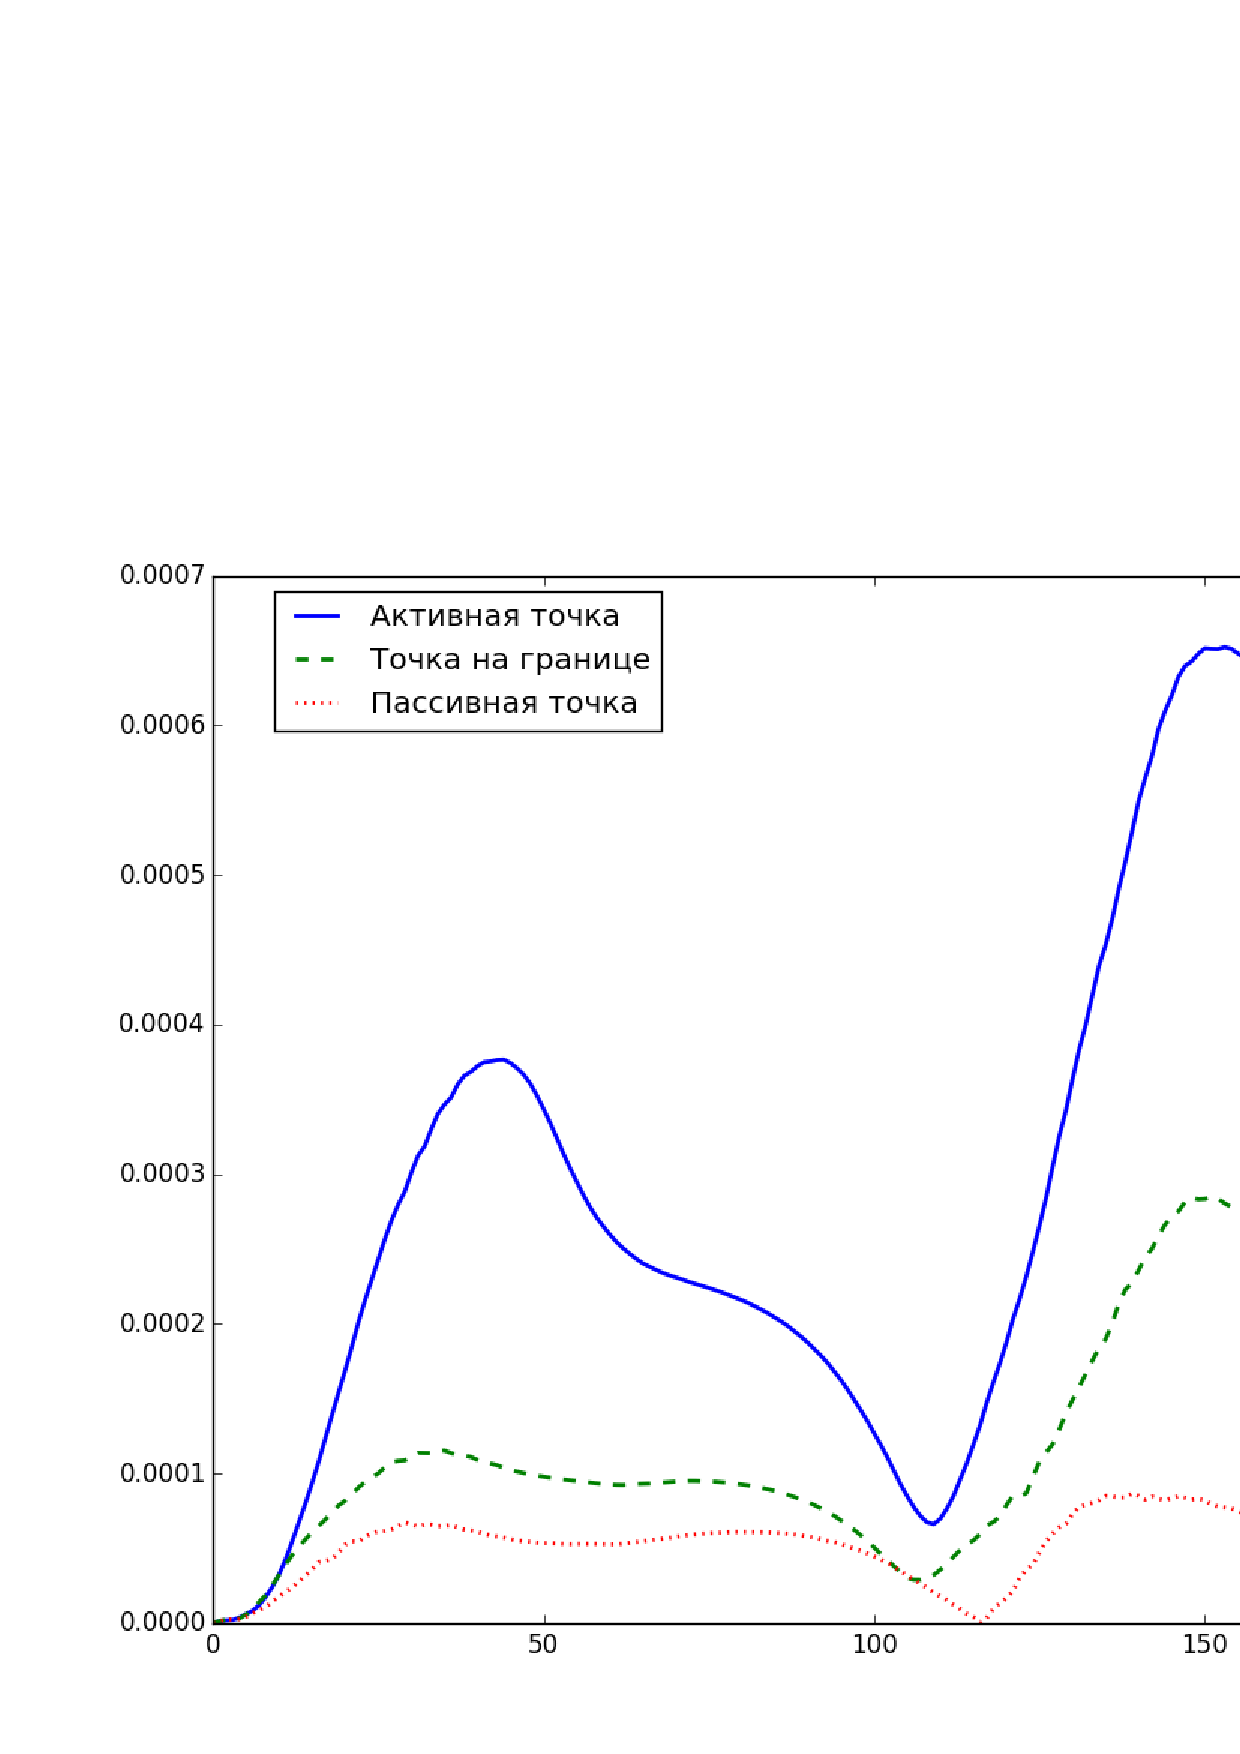
\includegraphics{forces.png}
\caption{\label{fig:fibrouse_forces}Зависимость напряжения от времени
для трех точек на фиброзном кольце}
\end{figure}

Как видно из рис. \ref{fig:fibrouse_forces}, качественно величина
напряжения для каждой точки демонстрирует схожую динамику изменения, но
при этом в области крепления и рядом с осями возникают большие
напряжения.

На рис. \ref{fig:pressure_limit} продемонстрировано, что в данной
конфигурации при завершении цикла работы клапан эффективно является
закрытым, т.к. в области его расположения резко изменяется давление и
скорость.

\begin{figure}[htbp]
\centering
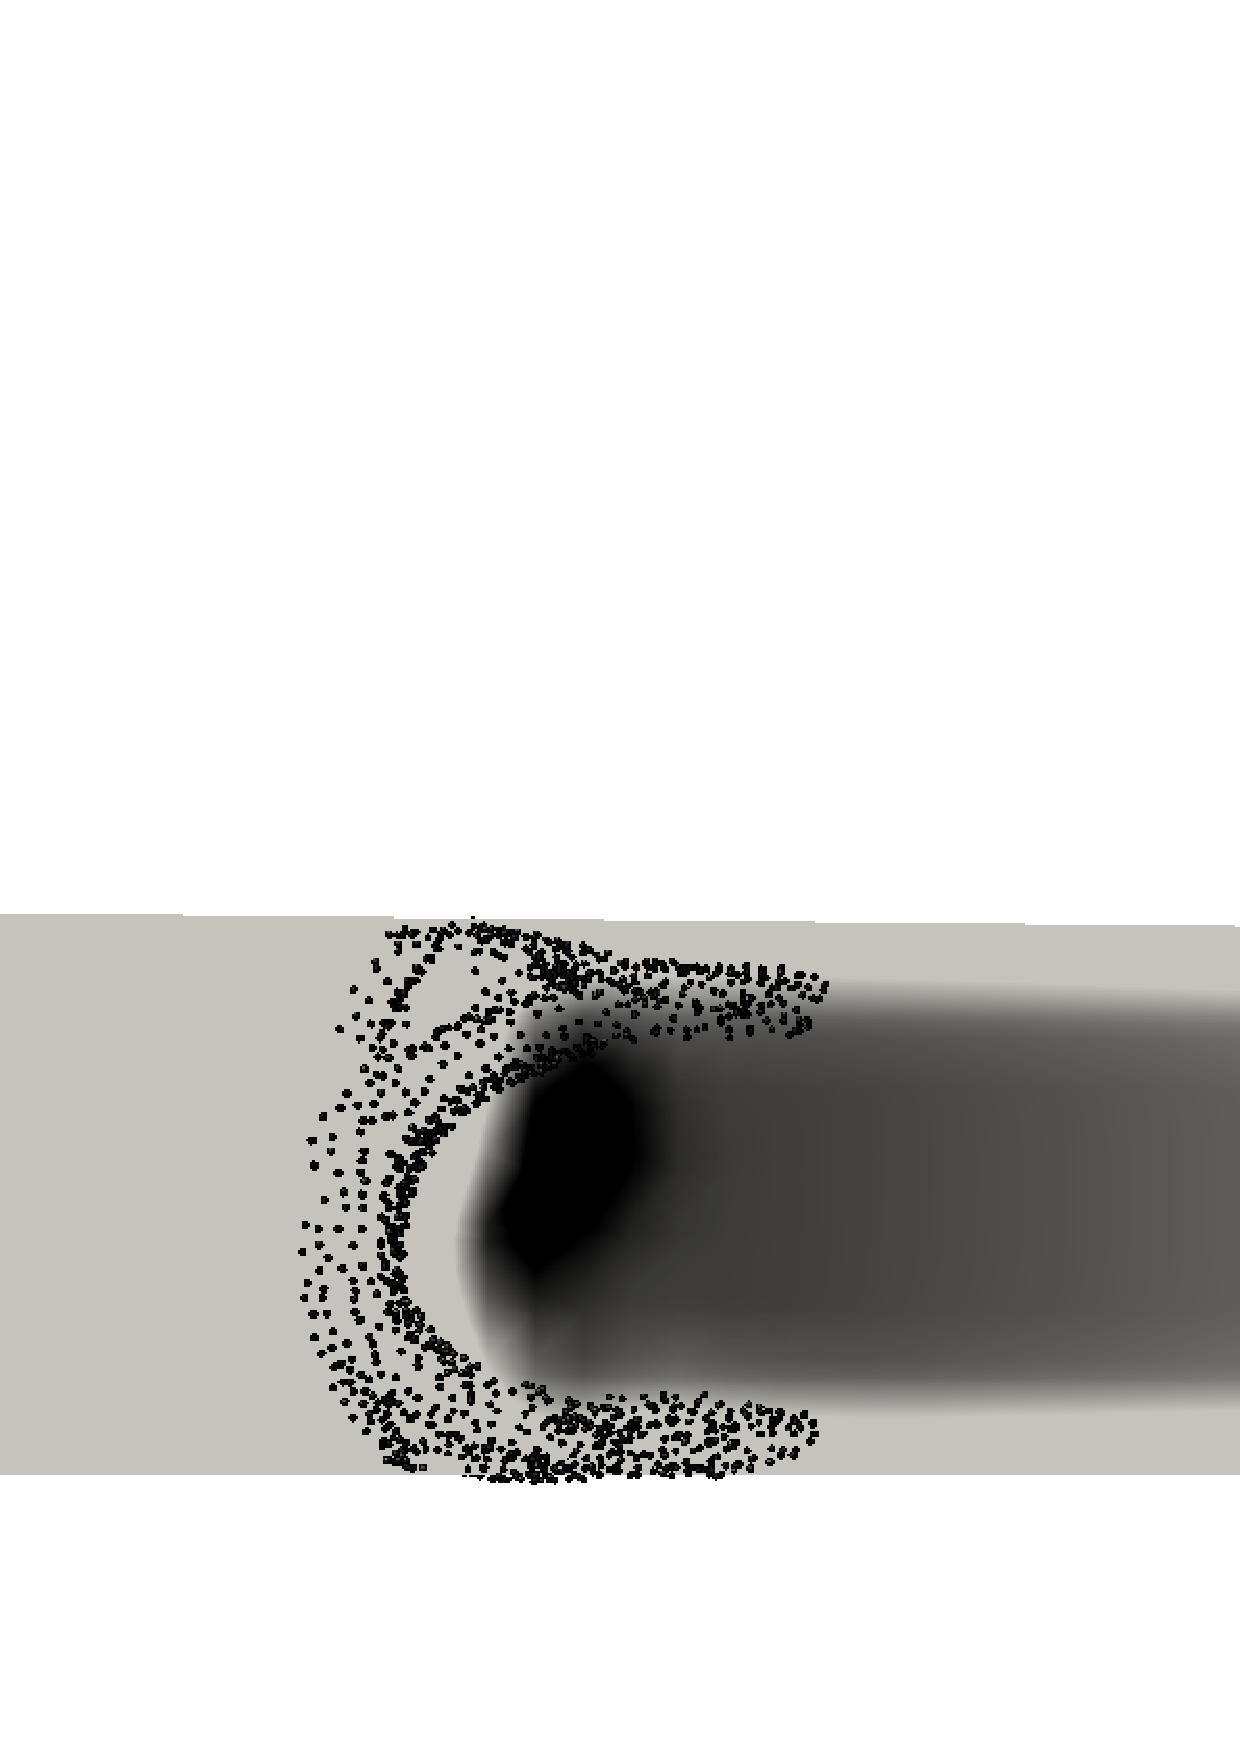
\includegraphics{pressure_limit.png}
\caption{\label{fig:pressure_limit}Резкий перепад давления при закрытии
клапана, точками обозначена поверхность фиброзного кольца}
\end{figure}

\section{Заключение}\label{ux437ux430ux43aux43bux44eux447ux435ux43dux438ux435}

Построенная модель работы искусственног сердечного клапана, учитывающая
течения крови с переменной плотностью и вязкостью, позволяет получать
физически непротиворечивые картины движения створок клапана для разных
геометрий.

\section*{Литература}\label{ux43bux438ux442ux435ux440ux430ux442ux443ux440ux430}
\addcontentsline{toc}{section}{Литература}

1.Association A.H. Heart disease and stroke statistics. 2015.

2.Institute D.C.R. Adult cardiac surgery database, executive summary.
2015.

3.Бокерия Л. et al. Механическое напряжение в створках митрального
клапана и биопротеза в митральной позиции. влияние геометрии фиброзного
кольца на величину напряжения створок. // Клиническая физиология
кровообращения. Научный центр сердечно-сосудистой хирургии им. АН
Бакулева РАМН, 2008. Vol. 2. Pp. 73--80.

4.Kim H.S. Nonlinear multi-scale anisotropic material and structural
models for prosthetic and native aortic heart valves. Georgia Institute
of Technology, 2009.

5.Taylor C.A., Hughes T.J., Zarins C.K. Finite element modeling of blood
flow in arteries // Computer methods in applied mechanics and
engineering. Elsevier, 1998. Vol. 158, № 1. Pp. 155--196.

6.Zhang Y., Bajaj C. Finite element meshing for cardiac analysis //
Univ. of Texas at Austin: ICES Technical Report. 2004.

7.Black M. et al. A three-dimensional analysis of a bioprosthetic heart
valve // Journal of Biomechanics. Elsevier, 1991. Vol. 24, № 9. Pp.
793--801.

8.Peskin C.S. The immersed boundary method // Acta numerica. Cambridge
Univ Press, 2002. Vol. 11. Pp. 479--517.

9.Griffith B.E. Immersed boundary model of aortic heart valve dynamics
with physiological driving and loading conditions // International
Journal for Numerical Methods in Biomedical Engineering. Wiley Online
Library, 2012. Vol. 28, № 3. Pp. 317--345.

10.Ma X. et al. Image-based fluid--structure interaction model of the
human mitral valve // Computers \& Fluids. Elsevier, 2013. Vol. 71. Pp.
417--425.

11.Gummel E. et al. Motion of viscous inhomogeneous incompressible fluid
of variable viscosity // Zbornik radova konferencije MIT. 2013. Pp.
2013--2014.

12.Geidarov N., Zakharov Y.N., Shokin Y.I. Solution of the problem of a
viscous fluid flow with a given pressure differential // Russian Journal
of Numerical Analysis and Mathematical Modelling. 2011. Vol. 26, № 1.
Pp. 39--48.

13.Dolgov D., Zakharov Y. Mathematical modelling of artificial heart
valve performance // `` Stability and control processes'' in memory of
vI zubov (sCP), 2015 international conference. IEEE, 2015. Pp. 518--521.

14.Dolgov D., Zakharov Y. Numerical modeling of artificial heart valve
// Mathematical modeling of technological processes. Springer, 2015. Pp.
33--43.

15.Каро К., others. Механика кровообращения. Мир, 1978.

16.Whitmore R.L. Rheology of the circulation. Pergamon, 1968.

17.Белоцерковский О.М. Численное моделирование в механике сплошных сред.
Наука. Гл. ред. физ.-мат. лит., 1984.

18.Яненко Н.Н. Метод дробных шагов решения многомерных задач
математической физики. Издательство`` Наукa'', Сибирское отделение,
1967.

19.Клышников К. et al. Сравнительная характеристика гидродинамических
показателей биопротезов клапанов сердца Юнилайн и Перикор // Клиническая
физиология кровообращения. 2013. P. 45.
